%\ProvidesFile{esapub.tex}[2001/04/25 1.1 (PWD)]
\documentclass[a4paper,twocolumn]{esapub2005} % European paper
\pagestyle{empty}

% introduce this option for the ESA publications style
\bibliographystyle{alpha}

\usepackage{times}
\usepackage{natbib}
\usepackage{amsmath}
\usepackage{graphicx}
\usepackage{textcomp}

\title{Optimal forward calculation method of the Marussi tensor due to a
       geologic structure at GOCE height}
\author[(1)]{Leonardo Uieda}
\author[(2,3)]{Everton P. Bomfim}
\author[(3)]{Carla Braitenberg}
\author[(2)]{Eder Molina}
\affil[(1)]{Observat\'orio Nacional, Rio de Janeiro, Brazil}
\affil[(2)]{Universidade de S\~ao Paulo, S\~ao Paulo, Brazil}
\affil[(3)]{Dipartimento di Geoscienze, Universit\`a di Trieste, Trieste, Italy}

\newcommand{\btx}{\textsc{Bib}\TeX}
\newcommand{\filename}{esapub}

\begin{document}

\keywords{GOCE; tesseroid; Marussi tensor}

\maketitle

\begin{abstract}
The new observations of GOCE present a challenge to develop new calculation methods
that take into account the sphericity of the Earth.
We address this problem by using a discretization with a series of tesseroids.
There is no closed formula giving the gravitational fields of the tesseroid and
numerical integration methods must be used, such as the Gauss Legendre Cubature (GLC).
A problem that arises is that the computation times with the tesseroids are high.
Therefore, it is important to optimize the computations while maintaining the desired accuracy.
This optimization was done using an adaptive computation scheme that consists of using a
fixed GLC order and recursively subdividing the tesseroids.
We have obtained an optimum ratio between the size of the tesseroid and its distance
from the computation point. Furthermore, we show that this size-to-distance ratio is
different for the gravitational attraction than for the gravity gradient tensor.
\end{abstract}

\section{Introduction}
The new gravity field observations of GOCE challenge the geophysical modeler to develop
new calculation methods that take into account the sphericity of the Earth.
The presently available forward modeling tools all use a Cartesian reference system,
which is sufficient for regional studies and for calculating the fields near the Earth's
surface.
On the other hand, this reference system is not ideal for calculating the fields at the
height of the satellite or for modeling global or continental areas \citep{smith_etal2001}.
We address this problem by discretizing the lithosphere with a series of tesseroids, or
spherical prisms.
Presently, there is no closed formula giving the gravitational fields of the tesseroid
and therefore numerical integration methods must be used.
We adopt the Gauss Legendre Cubature (GLC) integration method as in
\citet{asgharzadeh_etal2007}.
The GLC approximates the integration by a weighted sum over the integration limits and its
accuracy depends mainly on two factors.
First, the number of points used to discretize the integrand function, i.e. the GLC nodes.
Second, the distance from the computation point to the tesseroid relative to its size.
\\[0.2cm]
A problem that arises from numerical integration is that it makes the computation times
with the tesseroids quite high.
Therefore, it is important to optimize the calculation scheme while maintaining a desired
accuracy of the results.
This optimization can be done by either using an optimal number of GLC nodes or an optimal
size of the tesseroids.
\citet{ku1977} obtained a criteria that relates both options for the right rectangular
prism and vertical component of the gravitational attraction.
According to \citet{ku1977}, the distance from the prism to the computation point should
be greater than the distance between the GLC nodes.
Based on these results, \citet{li_etal2011} developed an adaptive computation approach that
consists of using a fixed GLC order and subdividing the tesseroids when the criteria of
\citet{ku1977} is breached.
A shortcoming of this approach is that it is not clear whether the results of \citet{ku1977}
are valid for the tesseroid and gravity gradient tensor.
\\[0.2cm]
To overcome this obstacle, we have obtained a similar criteria for the tesseroid and
the gravity gradient tensor.
In similar fashion to \citet{li_etal2011}, we have chosen to fix the number of GLC nodes
and investigate the optimum size of the tesseroid required to obtain a desired accuracy.
Furthermore, we have investigated whether this criteria is the same for the vertical
component of the gravitational attraction and for the components of the gravity gradient
tensor.


\section{Methodology}

Assuming a fixed the number of GLC nodes, the accuracy of the integration depends
only on the ratio between the largest dimension of the tesseroid (L) and the distance
from its top surface to the computation point (d).
In this scenario, an accurate result can be obtained by splitting the tesseroid
into smaller ones and calculating their combined effect.
The splitting can be done recursively until the resulting tesseroids are small
enough to achieve the desired accuracy.
Fig. \ref{fig:divide-scheme} shows a two-dimensional sketch of this computation scheme.

\begin{figure}[htb]
    \centering
        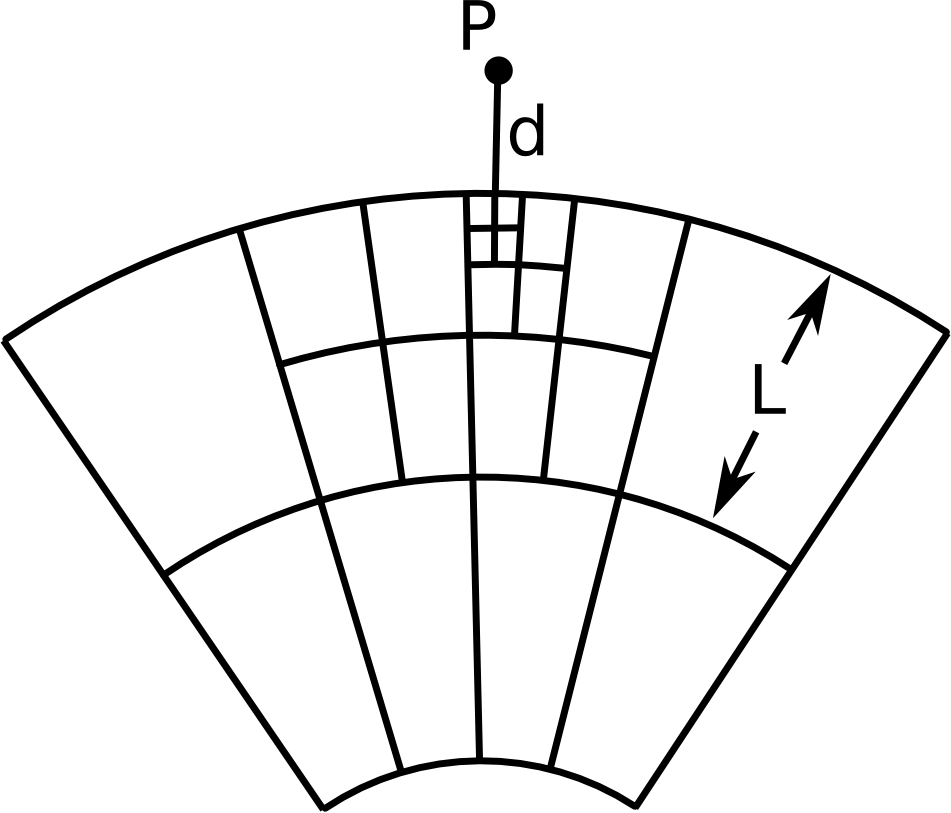
\includegraphics[width=\columnwidth]{../figures/divide-scheme.png}
    \caption{Sketch of the adaptive optimization algorithm. Recursively subdividing of
    tesseroids when the size-to-distance ratio is bellow a certain threshold.
    \label{fig:divide-scheme}}
\end{figure}

To determine the smallest size-to-distance ratio that yields results in the accuracy
expected from the GOCE observations and derived products, we must first establish a
reference to which we can compare the results of the GLC integration.
We chose a right rectangular prism with the same mass as the tesseroid as our reference.
The dimensions of the prism are related to the dimensions tesseroid by \citep{wild2008}:

\begin{equation}
\begin{split}
\Delta x &= \dfrac{r_1 + r_2}{2} \Delta \phi, \\
\Delta y &= \dfrac{r_1 + r_2}{2} \cos\left(\frac{\phi_1 + \phi_2}{2}\right) \Delta\lambda, \\
\Delta z &= \Delta r,
\end{split}
\label{eq:tess2prism}
\end{equation}

Eq. \ref{eq:tess2prism} results in a prism with approximately the same volume as the
tesseroid. Therefore, the density of the prism needs to be calculated to ensure that
the prism and tesseroid have the same mass:

\begin{equation}
\rho_p = \dfrac{V_t}{V_p} \rho_t
\label{eq:prismdens}
\end{equation}

where $V_t$ is the volume of the tesseroid and $V_p$ is the volume of the prism.
\\[0.2cm]
The right rectangular prism has closed formulas for the gravitational potential and its
first and second derivatives \citep{nagy2000}.
Since the gravitational effects of the tesseroid are calculated with respect to
the local reference frame of the computation point (Fig. \ref{fig:tess-coords}),
the gravitational attraction and gravity gradient tensor of the prism need to be
rotated to this reference frame before the comparisons can be made (Fig. \ref{fig:prism-coords}).
The rotation matrix used in this conversion is given in \citet{wild2008}.

\begin{figure}[htb]
    \centering
        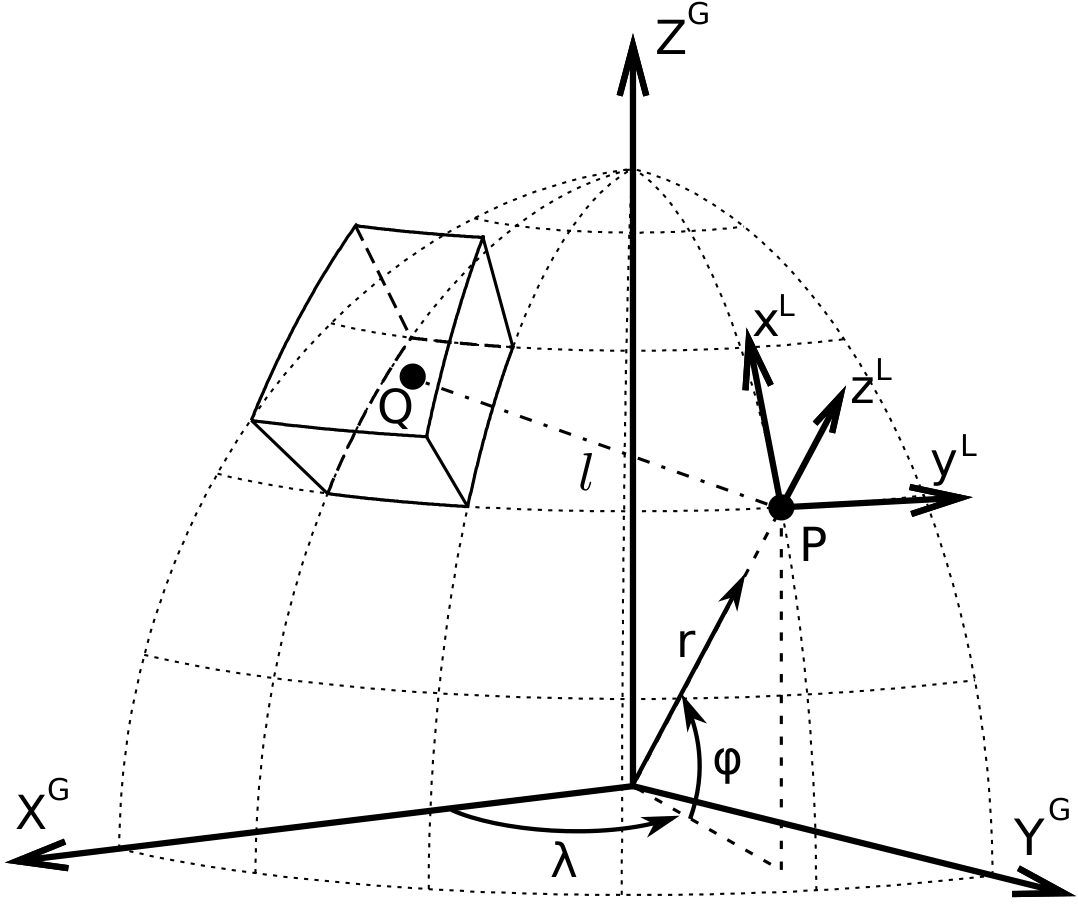
\includegraphics[width=\columnwidth]{../figures/tesseroid_coordsys_other.png}
    \caption{View of a tesseroid in the geocentric coordinate system. Point Q is an
    integration point. The computation point P is shown with its associated local
    coordinate system.
    \label{fig:tess-coords}}
\end{figure}
\begin{figure}[htb]
    \centering
        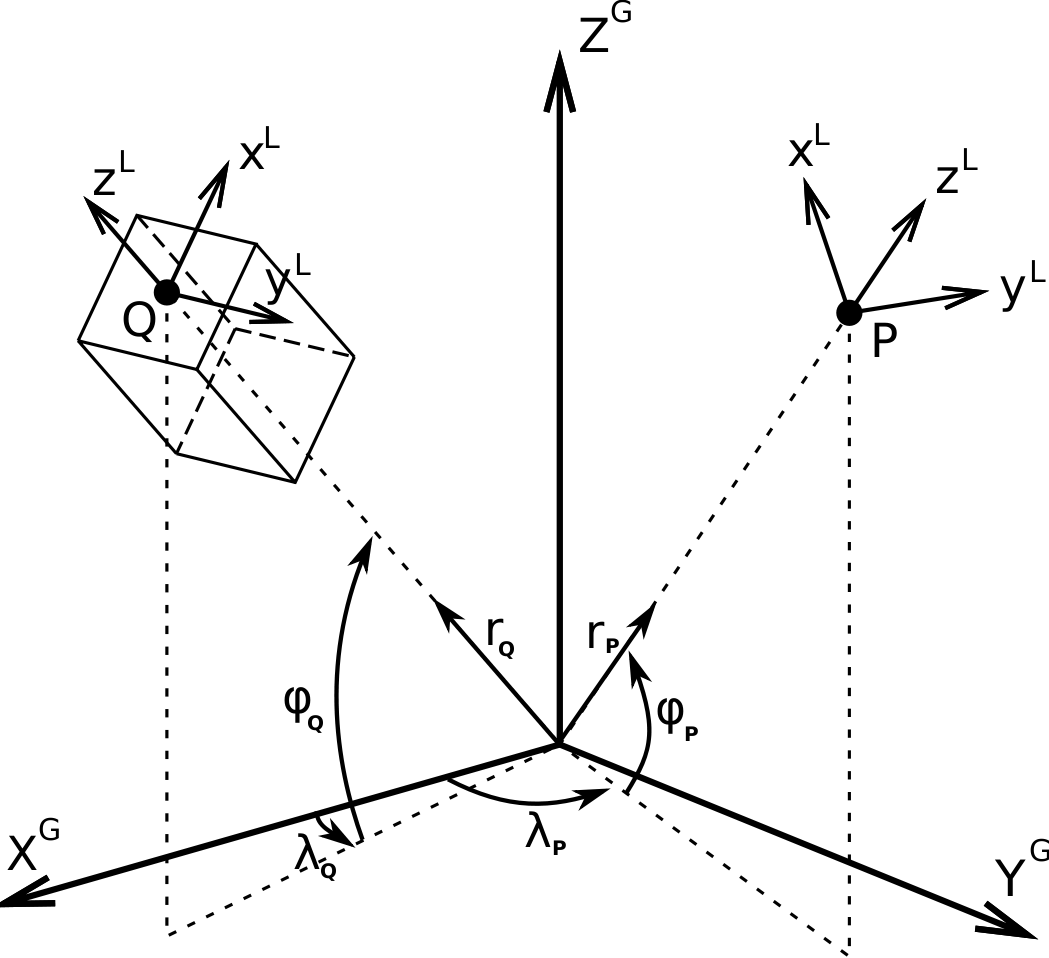
\includegraphics[width=\columnwidth]{../figures/coordinate_sys.png}
    \caption{A right rectangular prism shown in a geocentric reference frame.
    The computations are made with respect the local coordinate system associated
    with point Q. For the comparison with the effects of a tesseroid the computations
    must be rotated to local coordinate system associated with the computation point P.
    \label{fig:prism-coords}}
\end{figure}


\section{Results}

We have used a small tesseroid of size $0.001^{\circ} \times 0.001^{\circ} \times 100\ m$
in order to minimize the effect of the Earths curvature.
The number of GLC nodes was kept fixed at two nodes in each direction, resulting in a
total of eight nodes.
The vertical component of the gravitational attraction and six components of the gravity
gradient tensor were calculated on regular grids at heights ranging from 10 m to 2000 m.
Fig. \ref{fig:res-0.001} shows the absolute difference between the results of the
tesseroid and an equivalent prism against the size-to-distance ratio.
Fig. \ref{fig:res-0.001-profile} shows the same differences along a longitudinal
profile crossing the center of the tesseroid.
We assumed a desired accuracy of $10^{-2}$ mGal for $g_z$ and $10^{-3}$ E\"otv\"os for
the tensor components.
We found an optimum size-to-distance ratio for $g_z$ equal to one, which is accordance
with the results of \citet{ku1977}.
However, for the tensor components the optimum size-to-distance ratio found is four.
\\[0.2cm]
In order to check if the results obtained depend on the size of the tesseroid,
the same computations were repeated for a tesseroid of size
$0.0001^{\circ} \times 0.0001^{\circ} \times 10\ m$.
Fig. \ref{fig:res-0.0001} shows the differences against the size-to-distance ratio for
this tesseroid.
The ratio obtained for $g_z$ was slightly different (0.6) and the ratio for the tensor
components remained equal to four.
\\[0.2cm]
The optimum ratio obtained was used to implement the adaptive computation scheme of
\citet{li_etal2011} in the computer program \textit{Tesseroids} \citep{uieda_etal2010}.


\begin{figure*}[h]
    \centering
        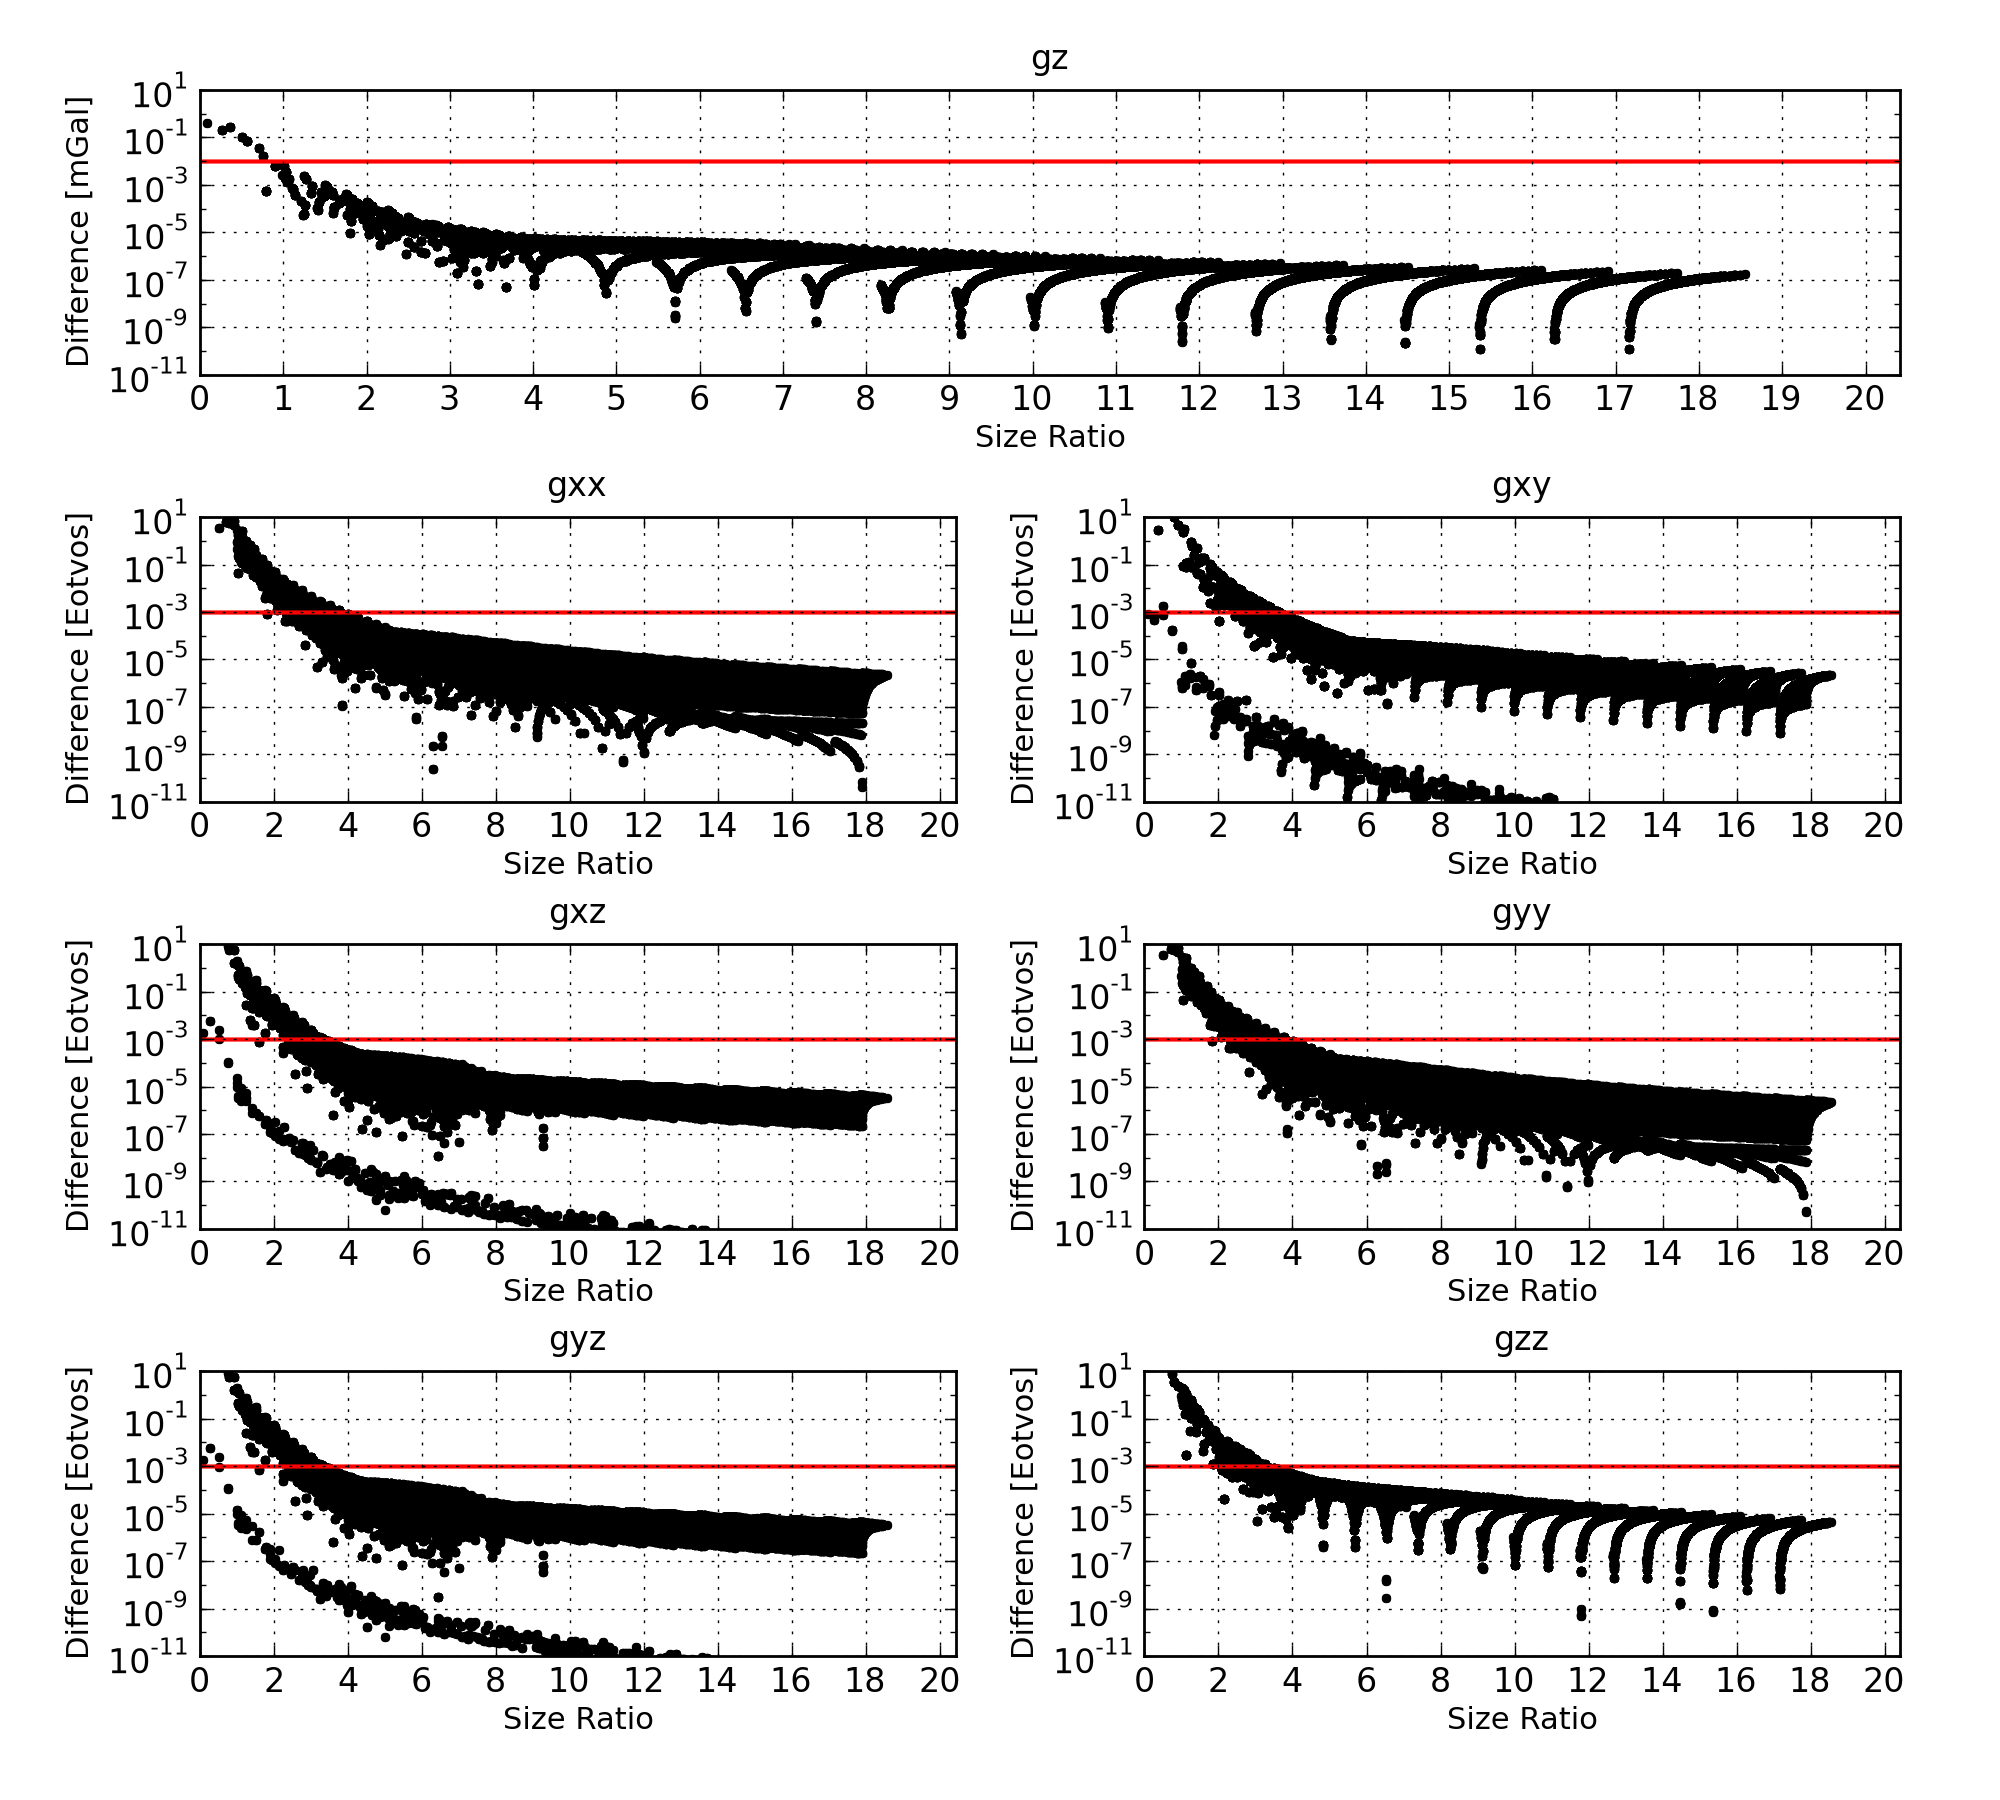
\includegraphics[width=\textwidth]{../figures/comparison0_001.png}
    \caption{Difference between gravitational effects of a tesseroid of size
    $0.001^{\circ} \times 0.001^{\circ} \times 100\ m$ and an equivalent prism.
    Red lines represent the desired accuracy.
    \label{fig:res-0.001}}
\end{figure*}
\begin{figure}[htb]
    \centering
        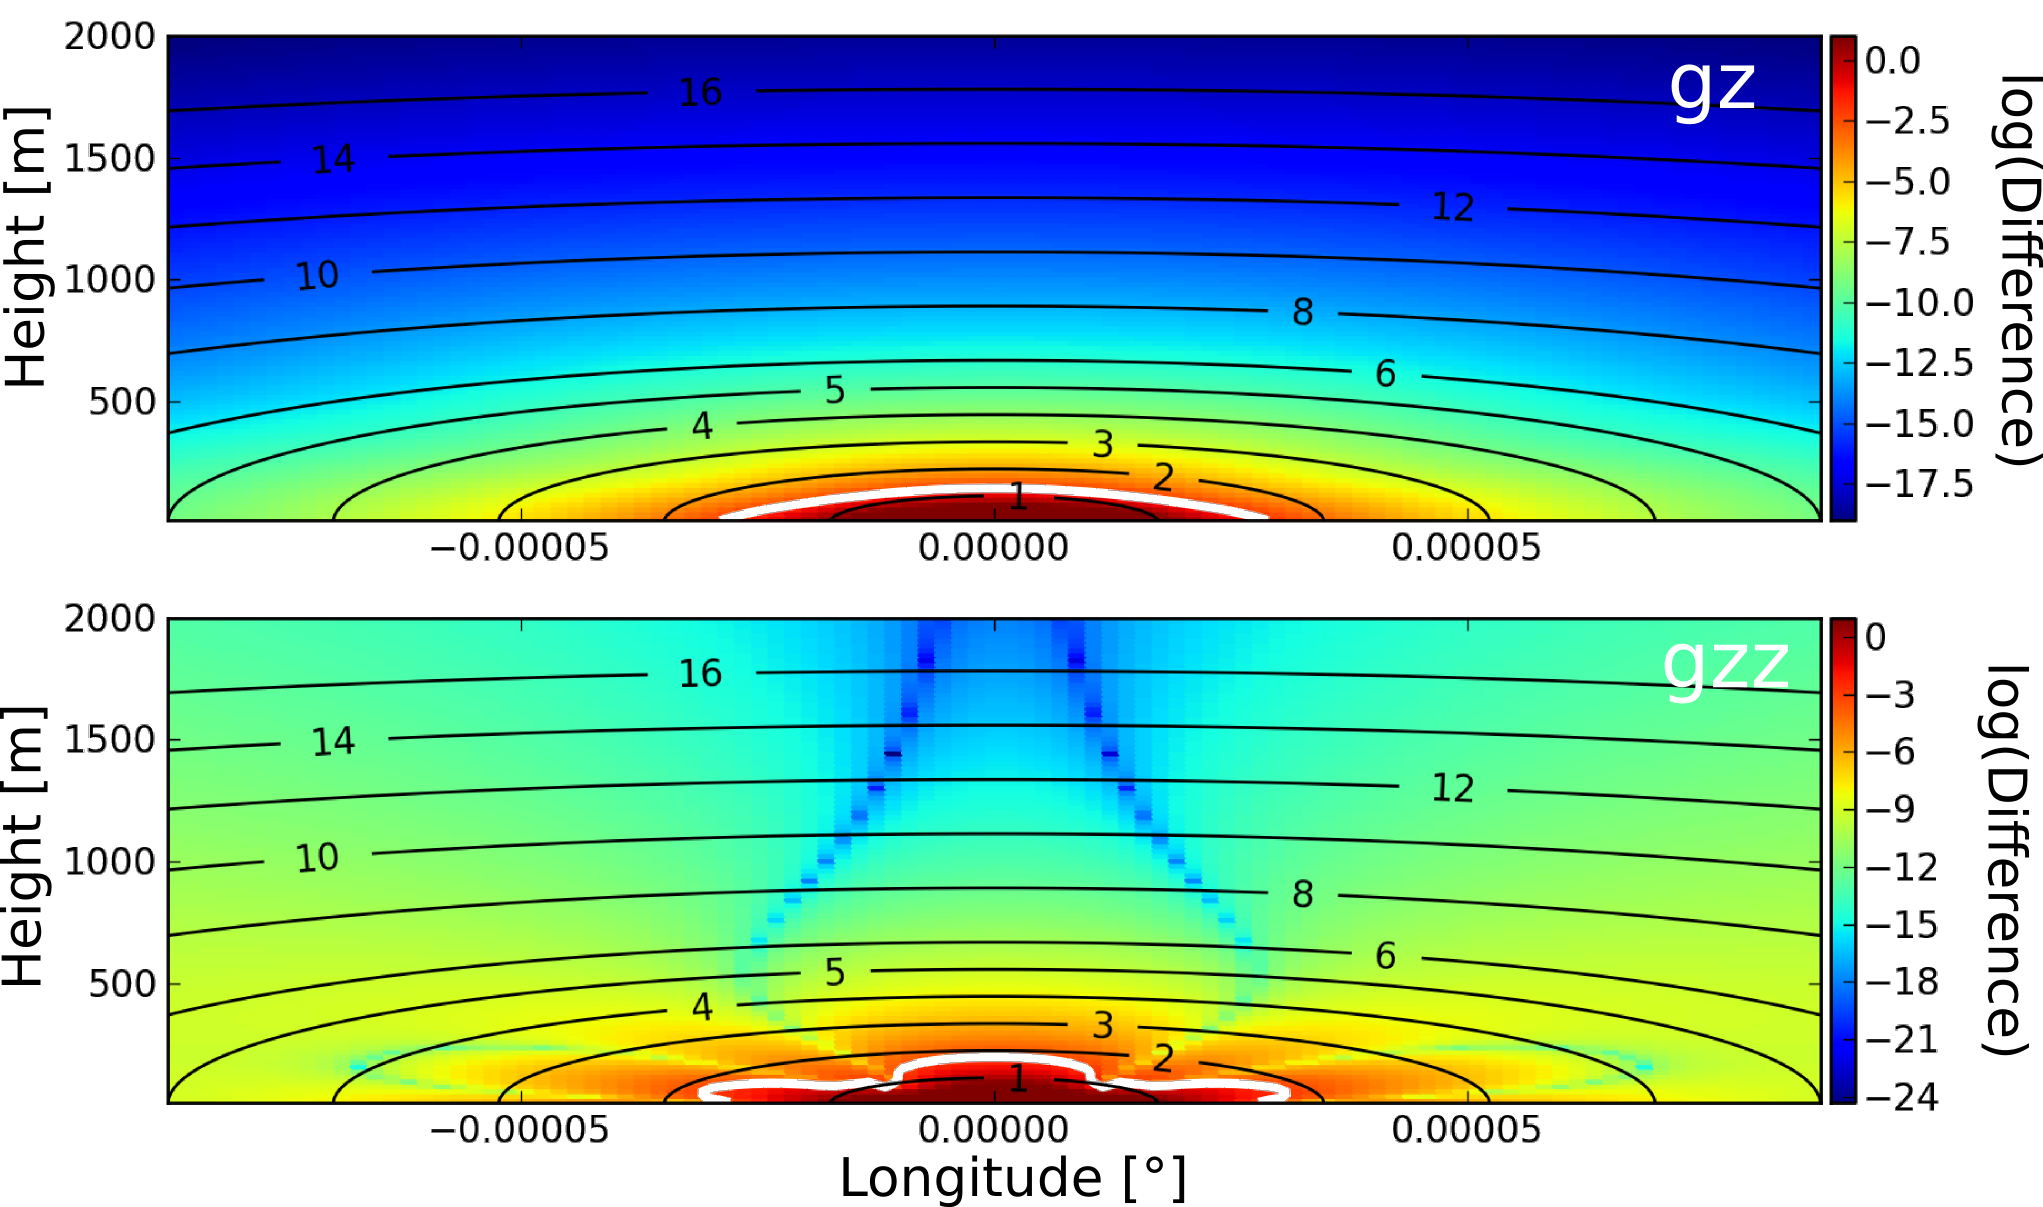
\includegraphics[width=\columnwidth]{../figures/comparion_profile_final.png}
    \caption{Logarithmic difference between gravitational effects of a tesseroid of
    size $0.001^{\circ} \times 0.001^{\circ} \times 100\ m$ and an equivalent prism
    along a longitudinal profile over the center of the tesseroid.
    White contour lines represent the desired accuracy. Black contour lines
    represent the size-to-distance ratio.
    \label{fig:res-0.001-profile}}
\end{figure}
\begin{figure*}[h]
    \centering
        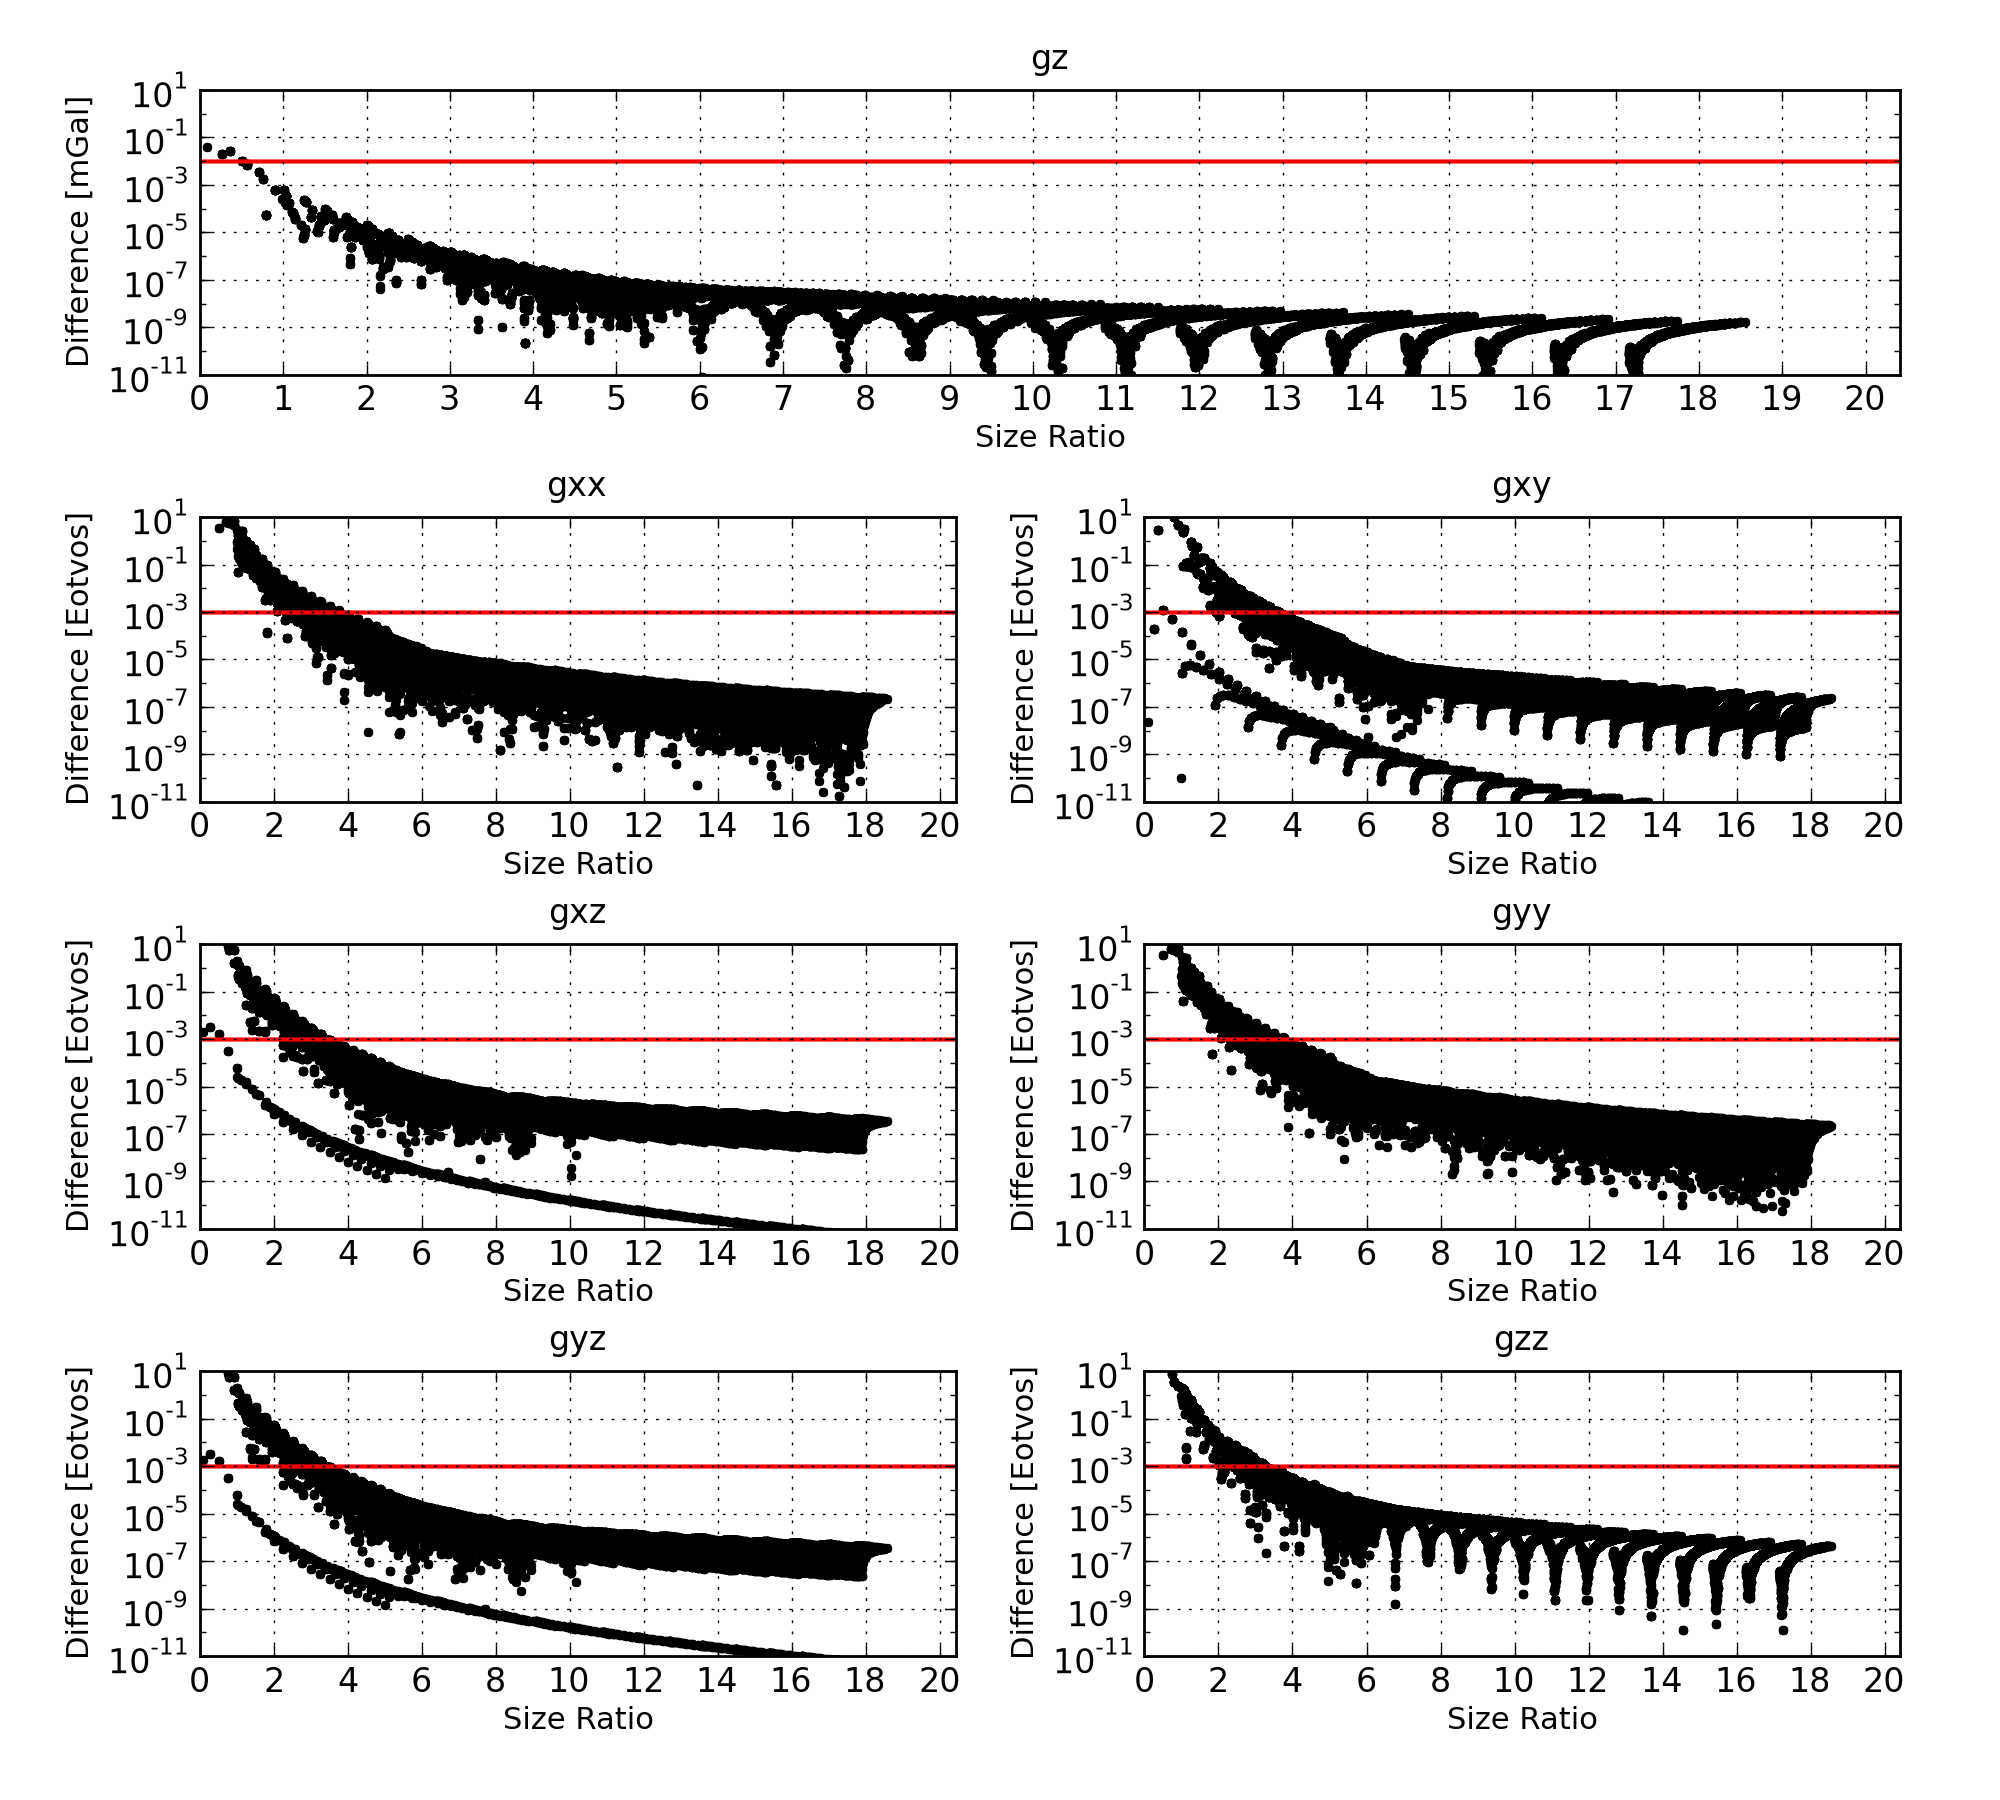
\includegraphics[width=\textwidth]{../figures/comparison0_0001.png}
    \caption{Difference between gravitational effects of a tesseroid of size
    $0.0001^{\circ} \times 0.0001^{\circ} \times 10\ m$ and an equivalent prism.
    Red lines represent the desired accuracy.
    \label{fig:res-0.0001}}
\end{figure*}

\section{Conclusions}

We have obtained an optimum size-to-distance ratio for the tesseroid.
The ratio found for the vertical component of the gravitational attraction agrees
with previous results.
However, the optimum ratio found for the tensor components is four times greater than
the one for the vertical component of the gravitational attraction.
This contradicts previous assumptions that the same ratio is valid for both derivatives
of the gravitational potential.
Furthermore, our results suggest that the optimum size-to-distance ratio does not depend
on the absolute size of the tesseroid.

\section*{Acknowledgments}

This research is made in cooperation with Valeria C.F. Barbosa from Observat\'orio
Nacional, Rio de Janeiro, Brazil, and in the frame of different projects:
PRIN2008, FAPESP, CAPES, GOCE-Italy.

\begin{thebibliography}{}

 \bibitem[Asgharzadeh et al.(2007)]{asgharzadeh_etal2007}
 Asgharzadeh, M.F., von Frese, R.R.B., Kim, H.R., Leftwich, T.E. \& Kim, J.W. (2007).
 Spherical prism gravity ef\mbox{}fects by Gauss-Legendre quadrature integration.
 \textit{Geophysics Journal International}, \textbf{169}, 1-11.

 \bibitem[Ku(1977)]{ku1977} Ku, C.C. (1977). A direct computation of gravity and magnetic
 anomalies caused by 2- and 3-dimensional bodies of arbitrary shape and arbitrary
 magnetic polarization by equivalent-point methot and a simplified cubic spline.
 \textit{Geophysics}, \textbf{42}, 610-622.

 \bibitem[Li et al.(2011)]{li_etal2011} Li, Z., Hao, T., Xu, Y. \& Xu, Y. (2011).
 An efficient and adaptive approach for modeling gravity effects in spherical coordinates.
 \textit{Journal of Applied Geophysics}, \textbf{73}, 221-231.

 \bibitem[Nagy et al.(2000)]{nagy2000} Nagy, D., Papp, G. \& Benedek, J. (2000).
 The gravitational potential and its derivatives for the prism.
 \textit{Journal of Geodesy}, \textbf{74}, 552-560.

 \bibitem[Smith et al.(2001)]{smith_etal2001} Smith, D.A., Robertson, D.S. \& Milbert, D.G.
 (2001). Gravitational attraction of local crustal masses in spherical coordinates.
 \textit{Journal of Geodesy}, \textbf{74}, 783-795.

 \bibitem[Uieda et al.(2010)]{uieda_etal2010} Uieda, L., Ussami, N. \& Braitenberg, C.F. (2010).
 Computation of the gravity gradient tensor due to topographic masses using tesseroids.
 \textit{Eos Transactions AGU}, \textbf{91}(26), Meeting of the Americas Supplement,
 Abstract G22A-04.

 \bibitem[Wild-Pfeif\mbox{}fer(2008)]{wild2008} Wilf-Pfeif\mbox{}fer, F. (2008).
 A comparison of different mass elements for use in gravity gradiometry.
 \textit{Journal of Geodesy}, \textbf{82}(10), 637-653.

\end{thebibliography}
\end{document}